\subsubsection{Pogon}
    Deluje na principu vzvodov in krivulj. Imamo glavno krivuljno 
    vreteno, ki se vrti sinhronizirano z pogonom glavnega vretena, 
    preko zobnikov s katerimi izbiramo, preko tabele, čas cikla enega 
    kosa, saj se za en obrat krivuljnega vretena izvede en cikel.

    Na spodnji sliki \ref{pogon} je v pogledu od zgoraj prikazana shema
    nekaterih delov eno-vretenske avtomatske stružnice.
    \begin{figure}[H]
        \begin{center}
            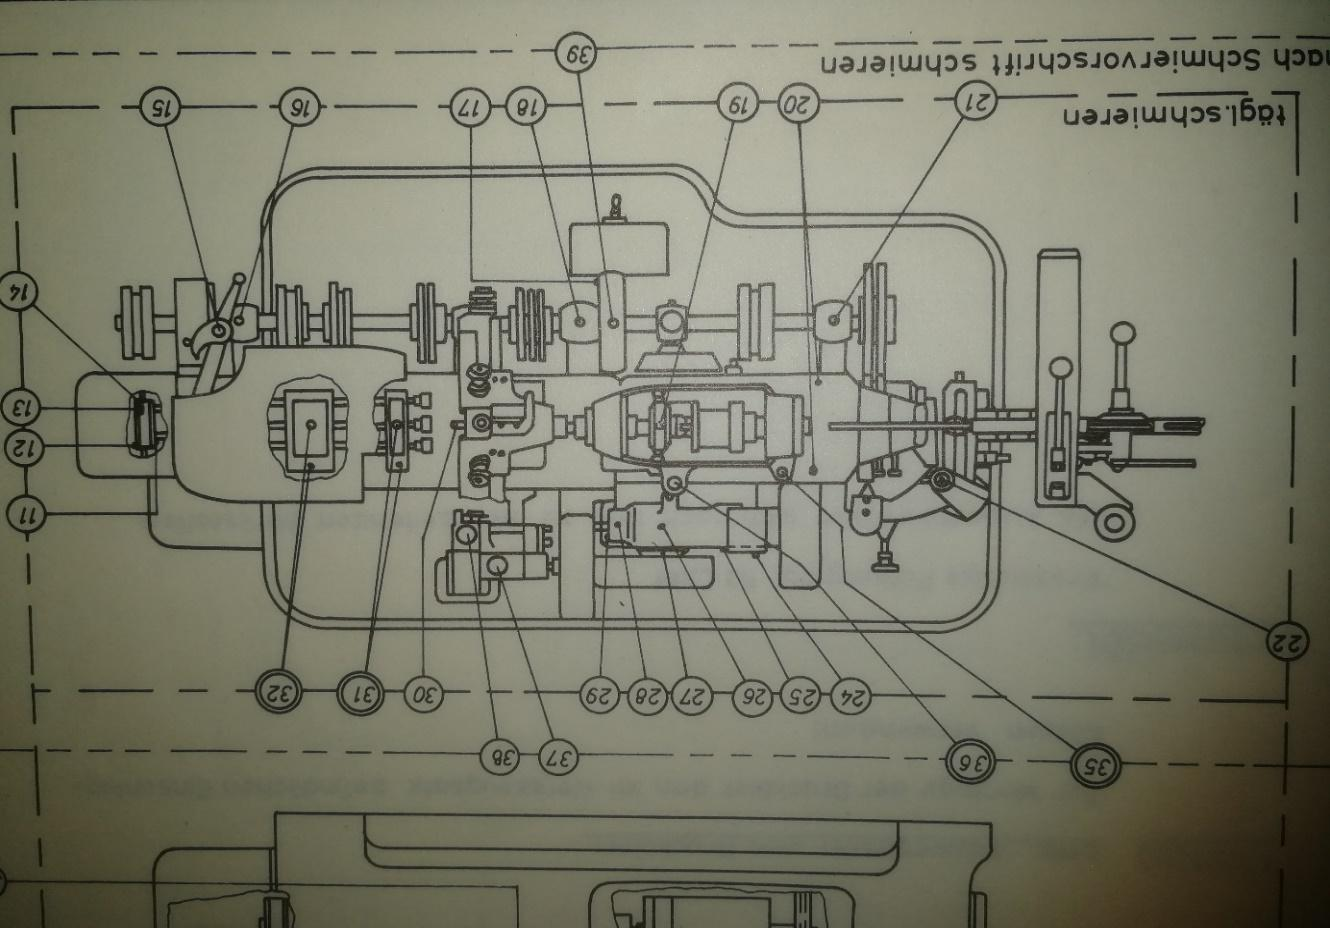
\includegraphics[width=\linewidth]{shema_avtomata.jpg}
            \caption{Shema delov eno-vretenske avtomatske stružnice
                    \cite{gauthier}}  
            \label{pogon} 
        \end{center}
    \end{figure}

    \noindent Za pogon se največkrat uporablja običajen trofazni elektromotor,
    ki preko menjalnika vrti glavno vreteno. Poznamo pa dve vrsti
    menjalnikov
    
    \begin{itemize}
        \item Avtomatski - z krivuljo lahko izbiramo med polno 
        hitrostjo, \( \frac{1}{2} \), \( \frac{1}{3} \), \( \frac{1}{4} \) 
        polne hitrosti ali pa zamenjamo 
        smer obratov (uporabno za vrezovanje navojev).

        \item Ročni- hitrost se nastavlja ročno z izbiro zobnikov 
        v menjalniku in se med obratovanjem ne more spreminjati.
    \end{itemize}
    \newpage

\subsubsection{Vpetje obdelovanca}
Avtomatske stružnice uporabljajo za vpetje izključno stročnice, 
saj so najnatančnejši in najhitrejši način vpetja. Edini problemi 
z stročnicami so, da se hitro zamažejo z ostružki, ki jo hitro 
uničijo. Njihov razpon vpetja je zelo majhen. V stročnico z 
izvrtino ø12 lahko vstavimo kos s premerom od ø11.5 do ø12.5, 
zato je potrebno menjati stročnico skoraj vedno, kadar se stroj nastavlja.
Poznamo dva načina vpetja pri avtomatih:
\begin{itemize}
    \item Dolgo-stružno: Sistem dveh stročnic, ki se vrtijo z 
    enakimi obrati. Sprednja stročnica- vodilna, kosa ne vpne, 
    ampak ga vodi, da ne opleta in se lahko struženje izvaja čim 
    bližje vpetju. Zadnja stročnica pa surovec vpne in ga podaja 
    skozi vodilno stročnico.
    \item Kratko-stružno: Sistem ene stročnice, ki vpne surovec
    ter ga ne vodi skozi vodilno stročnico tako, da struženje 
    poteka dlje od vpetja, kar se pri obdelovancih manjših 
    premerov pozna v ekscentričnosti stružnih površin in tudi v obdelavi.
    Večji kot je premer obdelovanca, dlje lahko gleda surovec iz stročnice.
\end{itemize}

Na spodnji sliki \ref{tipi_vodilnih_pus} je na levi strani prikazana
shema dolgo-stružne konfiguracije, na desni pa kratkostružna konfiguracija
stročnic na avtomatski stružnici.

\begin{figure}[H]
    \begin{center}
        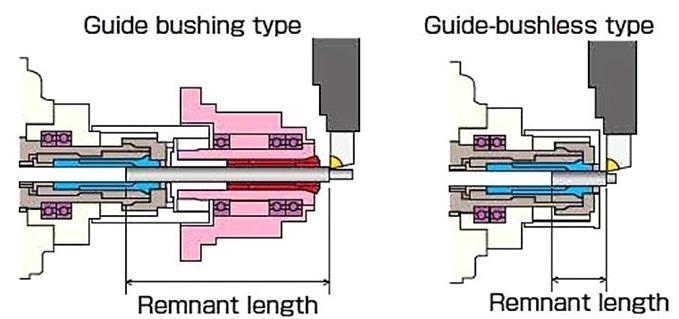
\includegraphics[width=\linewidth]{skuca_dolgo_struzenje.jpg}       
        \caption{Shema postavitve pri dolgem struženju z stročnicami
                \cite{interna}}
        \label{tipi_vodilnih_pus}
    \end{center}
\end{figure}

Prednosti dolgo-stružnih avtomatov je pa daljša dolžina struženja 
in boljše vpetje obdelovanca, zato je bolj primerna za daljše 
kose manjših premerov.

Prednost kratko-stružnih avtomatov je krajši ostanek in cenejši 
postopek, ker so vodilne stročnice veliko dražje od navadnih. 
Slabost pa je krajša dolžina struženja.

\subsubsection{Podajanje obdelovancev}
Za podajanje se uporabljajo podajalne naprave, ki podajajo 
obdelovanec z hidravliko ali pa z utežmi. Hidravlična podajalna 
naprava večinoma lahko sprejme več kot eno palico in jih tudi sama 
zamenja in vstavi v stroj. Možno je tudi nastavljati moč in dolžino
podajanja.

Spodaj, na sliki \ref{hidrobar_nalaganje}, je prikazan postopek
avtomatskega nalaganja novega obdelovanca v kanal hidrobara.
\begin{figure}[H]
    \begin{center}
        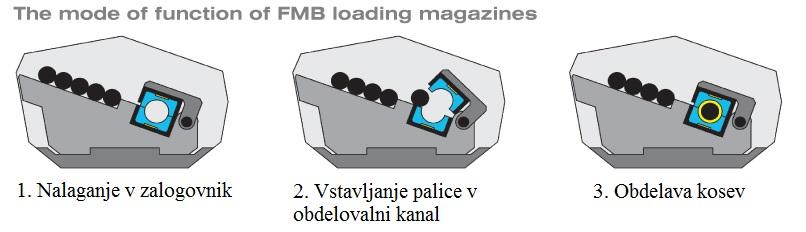
\includegraphics[width=15cm]{hidrobar_shema.jpg}
        \caption{Shema delovanja hidrobara
                \cite{interna}}   
        \label{hidrobar_nalaganje}
    \end{center}
\end{figure}

Obstajajo tudi podajalci, ki za vstavljanje palice uporabljajo 
utež. Ti so veliko cenejši in lažji za postavitev in nastavitev. 
Edina negativna stvar takšnih podajalcev je, da lahko naložimo v 
njih samo eno palico obdelovanca.
 
Na spodnji sliki \ref{shema_rocnega_podajalca} je prikazana shema 
delovanja ročnega podajalca palic.

\begin{figure}[H]
    \begin{center}
        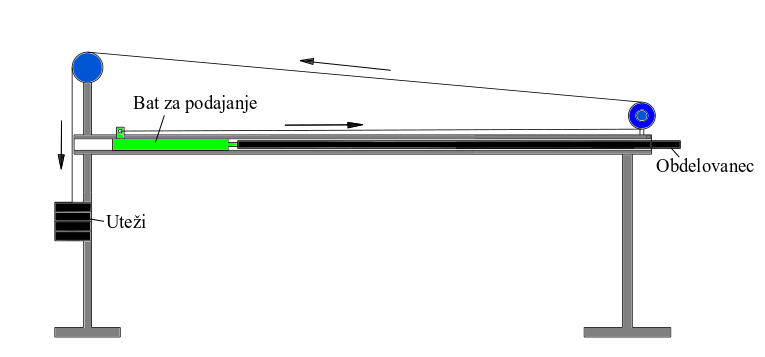
\includegraphics[width=15cm]{podajalec_utez.png}
        \caption{Ročni podajalec palic
                \cite{interna}}  
        \label{shema_rocnega_podajalca} 
    \end{center}
\end{figure}

\newpage

\subsubsection{Krivuljna gred}
Je krmilni del vsakega krivuljnega avtomata. Vsebuje krivulje, 
ki so največkrat iz kaljenega jekla, odpornega proti obrabi. Za en 
obrat krivuljnega vretena, se zaključi en cikel obdelovanja in je 
izdelan eden izdelek (Lahko tudi več, odvisno od nastavitve stroja). 
Hitrost obračanja se lahko spreminja z 
zobniki, imamo tudi že vnaprej pripravljeno tabelo, po kateri 
lahko izbiramo željeno hitrost in potrebne zobnike. Krivulje nato 
preko vzvodov premikajo prečne suporte, 
revolverske sani, vpenjajo obdelovanec… 

\noindent Poznamo dve vrsti krivulj:

\begin{itemize}
    \item Navadne - ploščate krivulje: uporabljamo za prečne pomike.
    \item Bobnaste krivulje: uporabljamo za vzdolžne pomike.
\end{itemize}

Krivuljna gred se lahko vklopi ali izklopi z pomočjo ročne sklopke,
ki se uporablja kadar se stroj nastavlja. Sklopka ima vgrajen 
zatič, ki se ob potencialnem strojelomu pretrga in ustavi vrtenje 
krivuljne gredi. Za izdelavo krivulj je potrebno veliko časa, saj 
se nenatančnosti geometrije poznajo na končnem izdelku. Zato je 
veliko krivulj standardiziranih in imajo vnaprej določen kot in 
višino vzpona in se lahko avtomat hitreje nastavi. Krivuljo po 
meri se izdeluje samo, če je serija kosov dovolj velika in če ni 
nikakršne druge možnosti.

\newpage
